% !TeX root = ../main.tex

\chapter{Introduction}\label{chapter:Introduction}

This chapter introduces the motivation behind this thesis, as well as giving an overview of existing work related to its topic.


\section{Motivation}

Ever since the dawn of video games, the focus has been largely on making virtual worlds look as real as possible. Advances in \gls{cga} techniques as well as continuously increasing processing power have allowed even real time \gls{cga} to become almost photo-realistic \autocite{photorealismRealtime}.
\newline
An example for this evolution in graphical fidelity is the comparison of \textit{id Software}'s \textit{Doom} video games from 1993 and 2016 in \autoref{fig:doom1993vs2016}. The basic way the game is played has stayed largely the same: Buttons on the keyboard trigger actions displayed on the screen, which acts as a window into the virtual world. The largest difference is the drastically more believable presentation of the game world.
\newline
The rise of high quality \gls{vra} however has allowed users to not only look into a virtual world, but to see it as if they were actually part of it. There are various factors which influence how effective the illusion of being part of a virtual environment is, however this thesis will focus on one, which is giving the user a fully animated body, as ''a virtual body in the context of a head-mounted dis-play based virtual reality is a critical contributor to the sense of being in the virtual location'' \autocite[p.~374]{senseEmbodimentVR}
\newline
A problem that arises when giving the user a body is that the virtual world can influence the virtual body, that is to say exert forces on it, but not on the real body of the user. This can result in situations where the real and virtual body are mismatched, due to, for example, the tracked position of a real hand being inside a virtual object, such as a wall.
\todo {rubber hand easy fool blabla \autocite{rubberHandsFeel}}



\begin{figure}[!tbp]
  \centering
  \subfloat[Doom1993][Doom 1993 \autocite{gamestarDoomPics}]{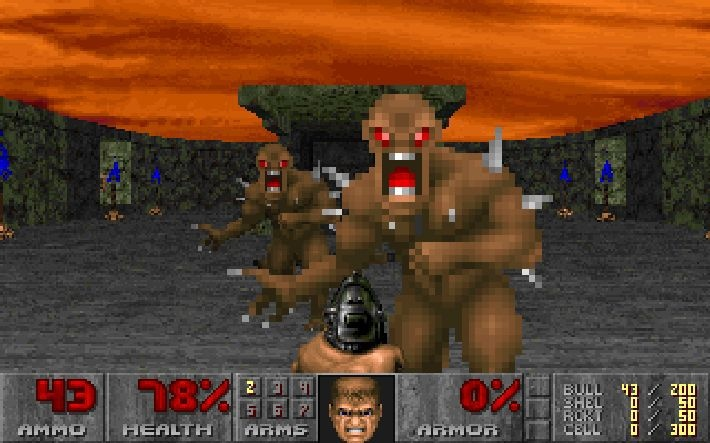
\includegraphics[height=0.2\textheight]{figures/doom1993.jpg}\label{fig:doom1993}}
  \hfill
  \subfloat[Doom2016][Doom 2016 \autocite{newGameNetworkDoomPics}]{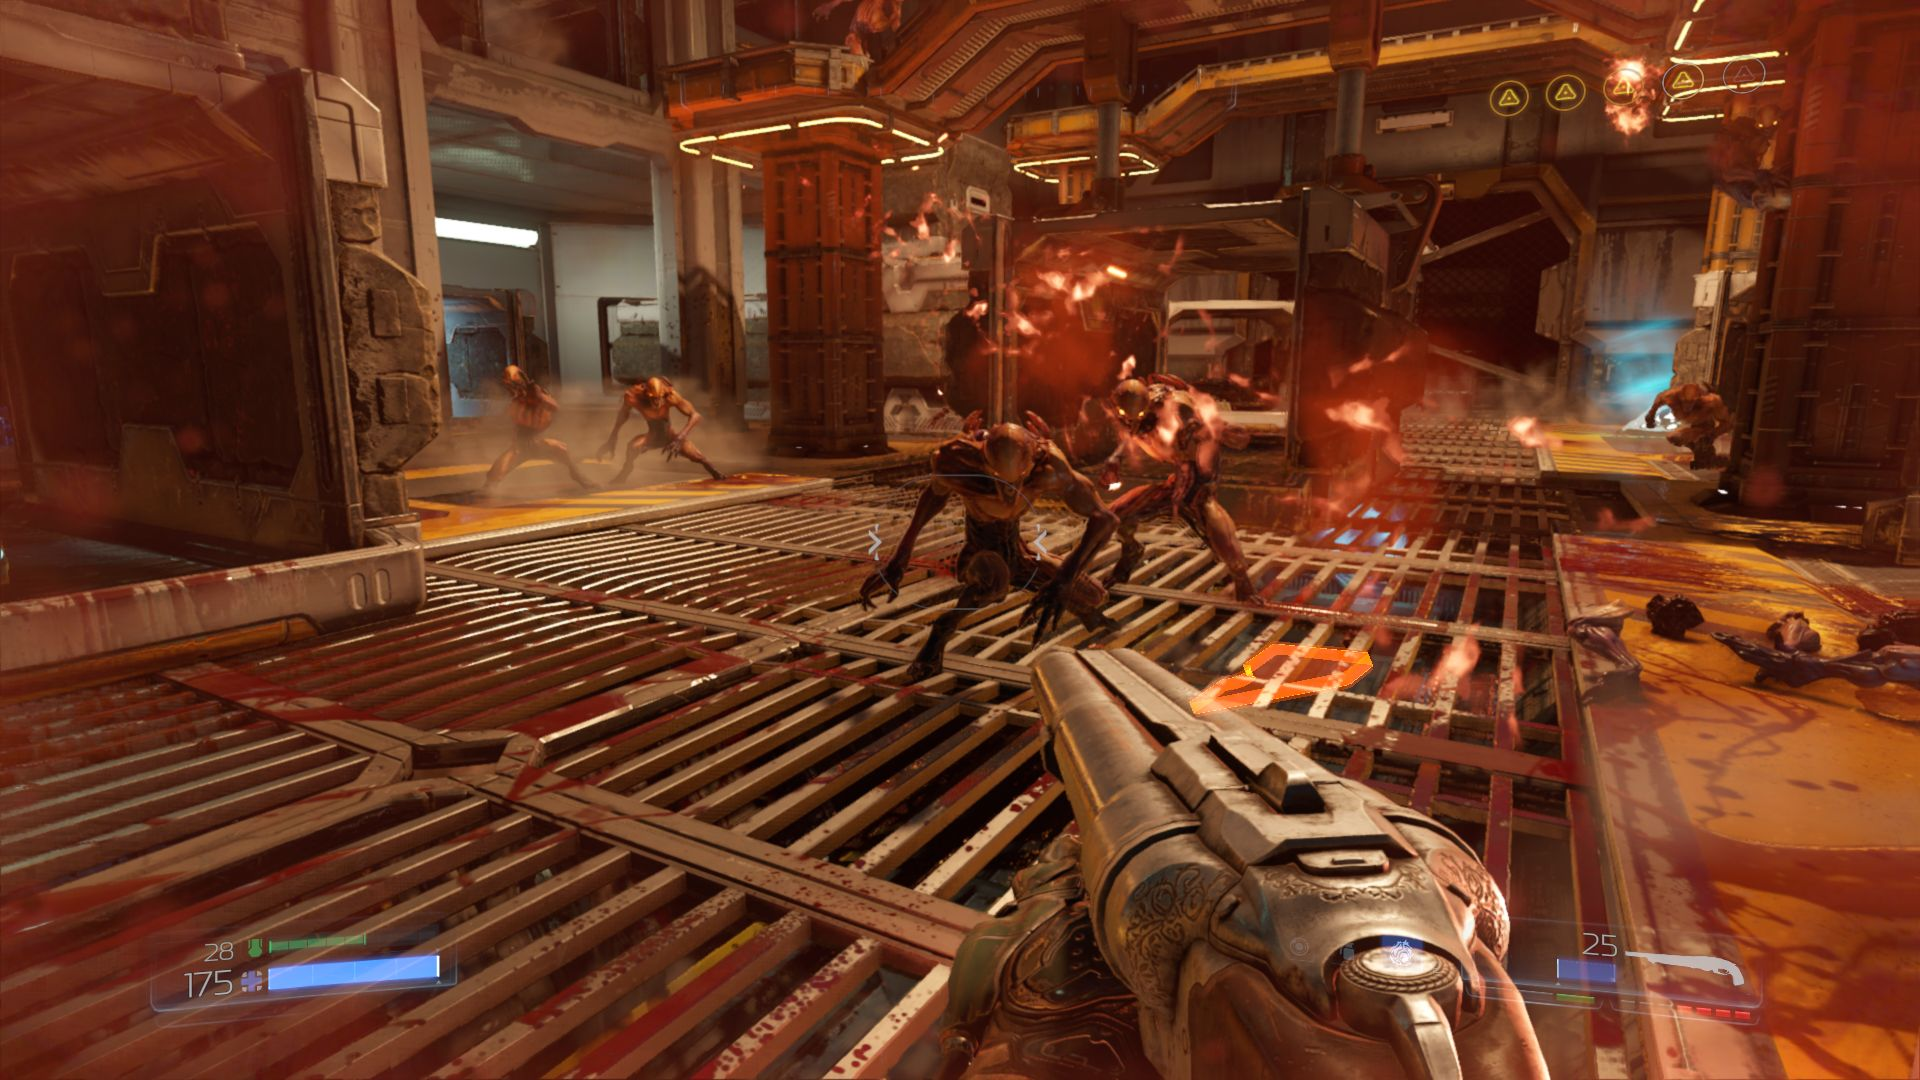
\includegraphics[height=0.2\textheight]{figures/doom2016}\label{fig:doom2016}}
  \caption{Evolution of \gls{cga} exemplified by \textit{Doom} games}
  \label{fig:doom1993vs2016}
\end{figure}


\section{Related Work}